\section{Model mismatch: $k$-component graph}

In many applications, specially those in fully automated and unsupervised settings,
the number of clusters is either unknown or it needs to be inferred from the data.
In this section we consider an experiment involving model mismatch: the underlying
Laplacian matrix that generates the data has $K$ number of components but we actually
use $J$, $J < K$, number of components to estimate it.
Additionally, we consider that the generative model is noisy, i.e.,
$\mathbf{L}_{\mathsf{noisy}} = \mathbf{L}_{\mathsf{bm}} + \mathbf{L}_{\mathsf{ER}}$,
where the parameters of the Erdos-Renyi model that acts as noise are $p = 0.25$ and
$\kappa = 0.45$. The block-model $\mathbf{L}_{\mathsf{bm}}$ is constructed with seven
blocks, each of which with seven nodes that are fully connected among themselves. The
weights on the edges are drawn from $\mathsf{Uniform}(0, 1)$.

\begin{figure}[!htb]
    \centering
    \begin{subfigure}[b]{0.3\textwidth}
        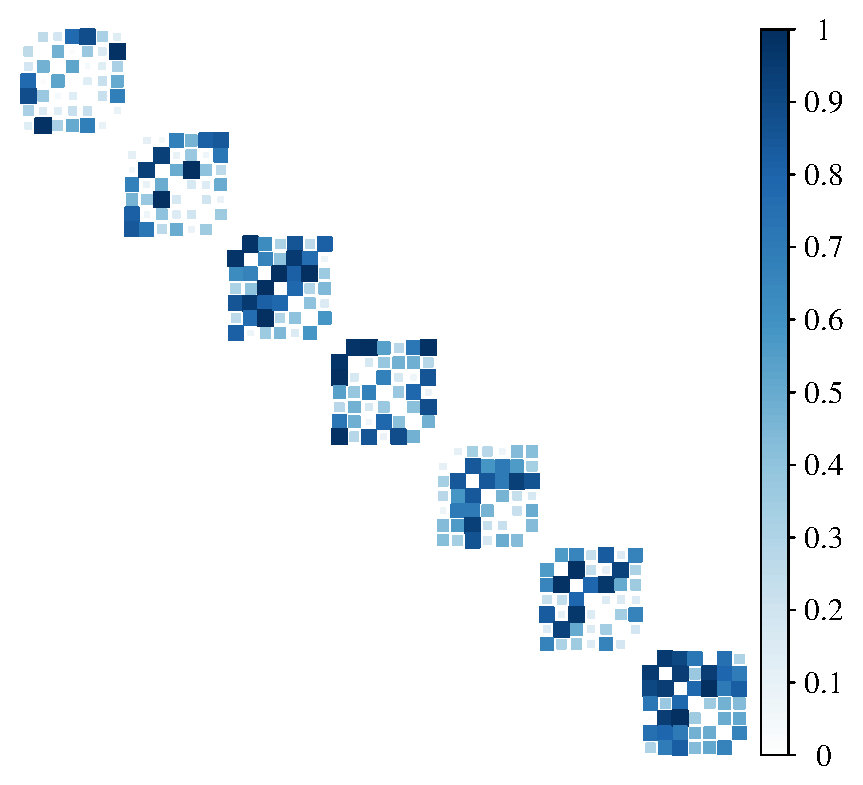
\includegraphics[width=\textwidth]{model-mismatch/true_mat.eps}
        \caption{Ground Truth Laplacian}
    \end{subfigure}
    ~ %add desired spacing between images, e. g. ~, \quad, \qquad, \hfill etc.
      %(or a blank line to force the subfigure onto a new line)
    \begin{subfigure}[b]{0.3\textwidth}
        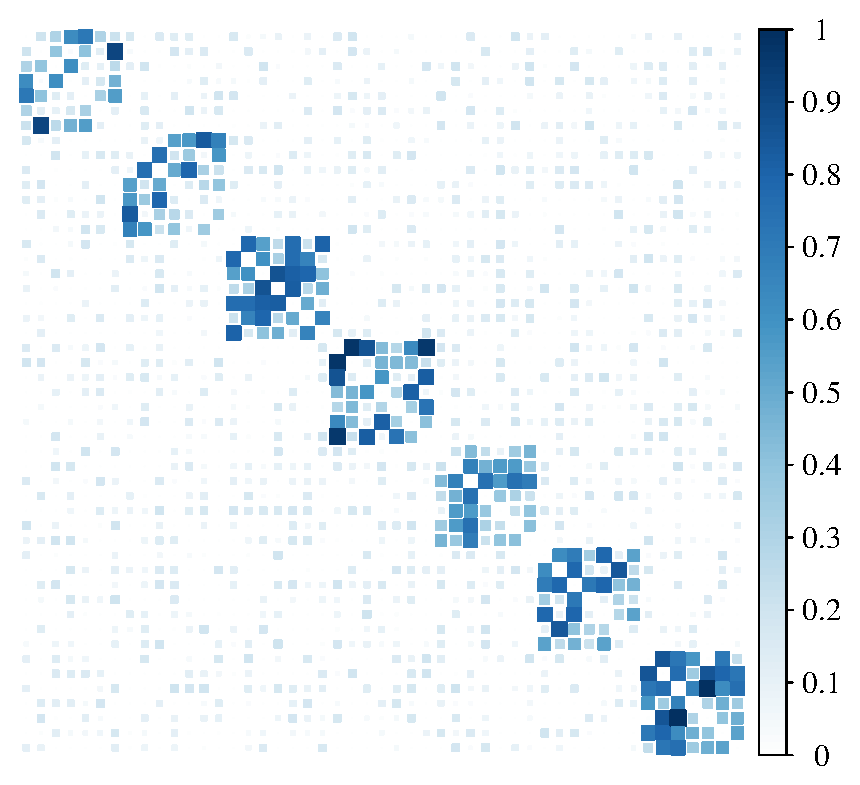
\includegraphics[width=\textwidth]{model-mismatch/noisy_mat.eps}
        \caption{Noisy Laplacian matrix}
    \end{subfigure}
    ~ %add desired spacing between images, e. g. ~, \quad, \qquad, \hfill etc.
    %(or a blank line to force the subfigure onto a new line)
    \begin{subfigure}[b]{0.3\textwidth}
        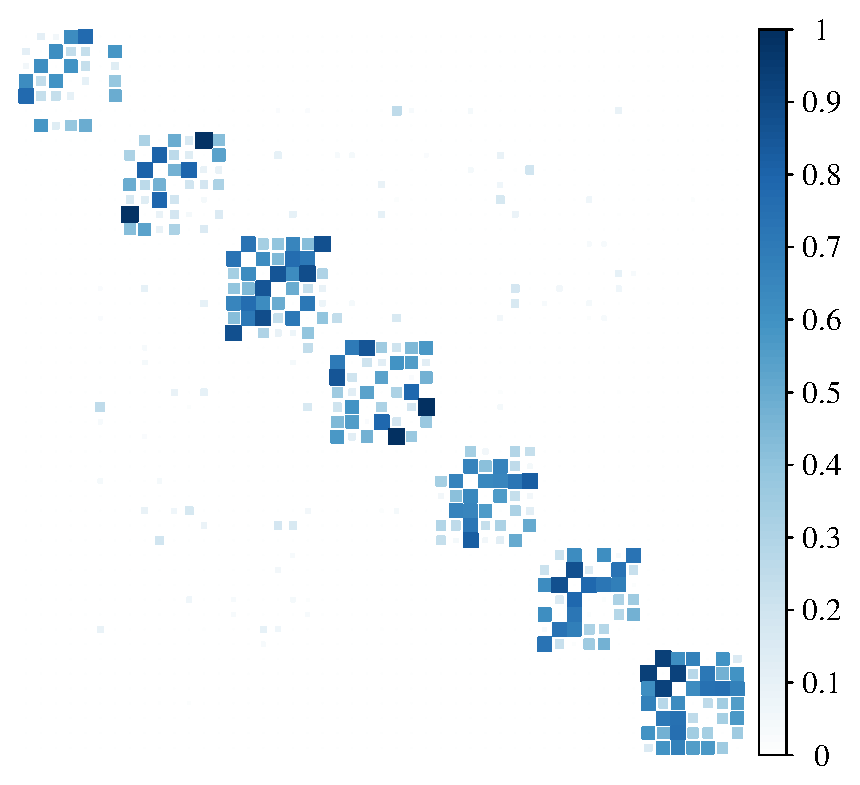
\includegraphics[width=\textwidth]{model-mismatch/est_mat.eps}
        \caption{Learned Laplacian ($K = 2$)}
    \end{subfigure}
        \\
    \begin{subfigure}[b]{0.3\textwidth}
        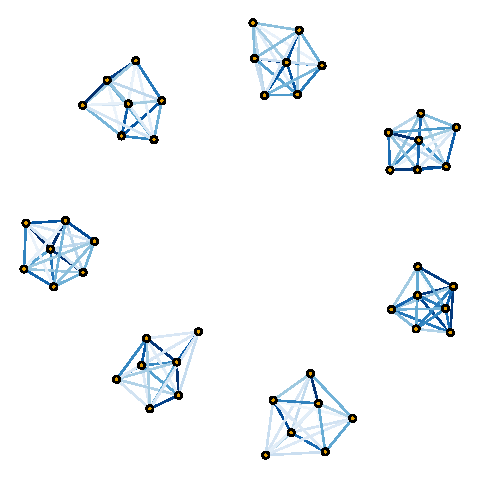
\includegraphics[width=\textwidth]{model-mismatch/true_graph.eps}
        \caption{Ground Truth graph}
    \end{subfigure}
    ~ %add desired spacing between images, e. g. ~, \quad, \qquad, \hfill etc.
      %(or a blank line to force the subfigure onto a new line)
    \begin{subfigure}[b]{0.3\textwidth}
        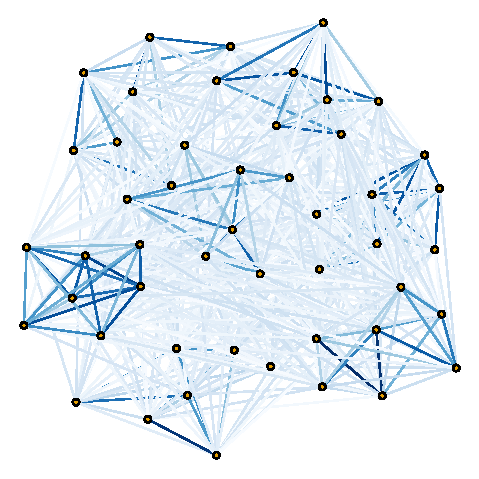
\includegraphics[width=\textwidth]{model-mismatch/noisy_graph.eps}
        \caption{Noisy graph}
    \end{subfigure}
    ~ %add desired spacing between images, e. g. ~, \quad, \qquad, \hfill etc.
    %(or a blank line to force the subfigure onto a new line)
    \begin{subfigure}[b]{0.3\textwidth}
        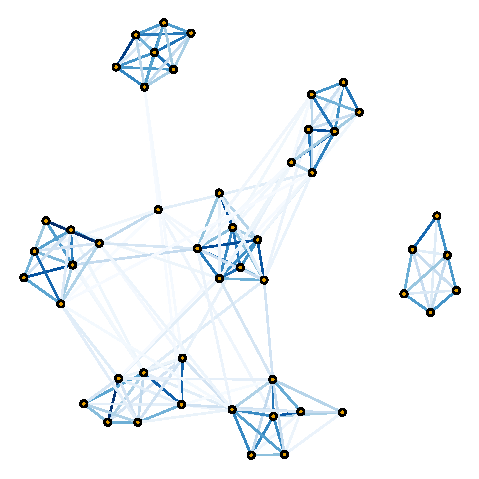
\includegraphics[width=\textwidth]{model-mismatch/est_graph.eps}
        \caption{Learned graph}
    \end{subfigure}
        \caption{Example of model mismatching. (a) the ground truth graph Laplacian of a seven-component graph
                 ($\mathbf{L}_{\mathsf{true}}$), (b) $\mathbf{L}_{\mathsf{true}}$ after being corrupted by noise,
                 (c) the learned graph Laplacian with a performance of
                 $(\mathsf{RE}, \mathsf{FS}) = (0.18, 0.81)$.
                 The panels (d), (e), and (f) correspond to the graphs represented by the Laplacian matrices in
                 (a), (b), and (c), respectively.}
        \label{fig:7-comp-graph}
\end{figure}

\begin{figure}[!htb]
  \centering
  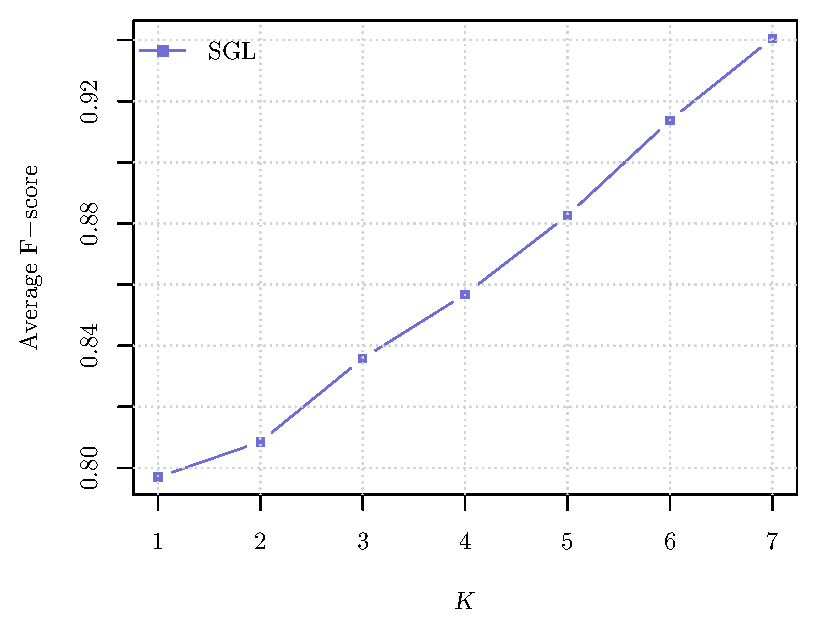
\includegraphics[width=\textwidth]{model-mismatch/fscore.eps}
  \caption{F-score as a function of the number of components $K$.}
  \label{fig:fscore-k}
\end{figure}

